\documentclass[a4paper, 12pt]{article}
\usepackage{geometry}
\geometry{a4paper,
total={170mm,257mm},left=2cm,right=2cm,
top=2cm,bottom=2cm}

\usepackage{mathtext}
\usepackage{amsmath}
\usepackage[T2A]{fontenc}
\usepackage[utf8]{inputenc}
\usepackage[english,russian]{babel}
\usepackage{graphicx, float}
\usepackage{tabularx, colortbl}
\usepackage{caption}
\captionsetup{labelsep=period}

\newcommand{\parag}[1]{\paragraph*{#1:}}
\DeclareSymbolFont{T2Aletters}{T2A}{cmr}{m}{it}
\newcounter{Points}
\setcounter{Points}{1}
\newcommand{\point}{\arabic{Points}. \addtocounter{Points}{1}}
\newcolumntype{C}{>{\centering\arraybackslash}X}

\author{Калинин Даниил, Б01-108}
\date{\today}
\title{Лабораторная работа 5.4.1}

\begin{document}
\maketitle
\parindent=0cm

\parag {Цель работы}
Измерить пробег $\alpha$-частиц в воздухе двумя способами и определить энергию частиц.

\parag {В работе используются}
торцевой счётчик Гейгера, сцинтилляционный счётчик.

\parag {Теоритическая справка} ~\\

Явление радиоктивности состоит в самопроизвольном распаде ядер с испусканием одной или нескольких частиц. К числу радиоактивных процессов относятся $\alpha$- и $\beta$-распады (в том числе и $K$-захват), $\gamma$-излучение, деление ядер, а также испускание запаздывающих нейтронов и протонов. В нашей работе мы будем рассматривать первое явление.

При $\alpha$-распаде исходное родительское ядро испускает ядро гелия ($\alpha$-частицу) и превращается в дочернее ядро, число протонов и нейтронов которого меньше на две единицы. Функциональная связь между энергией $\alpha$-частицы $E$ и периодом полураспада радиоактивного ядра $T_{1/2}$ хорошо описывается формулой:

\begin{equation}
    lg T_{1/2} = \frac{a}{\sqrt{E}} + b
\end{equation}

Экспериментально энергию $\alpha$-частиц удобно определять по величине их пробега в веществе. Они, главным образом, теряют свою энегрию от неупругих столкновений с атомами вещества. Эти столкновения вызывают ионизацию и возбуждение атомов, поэтому такие потери называются ионизационными. 

В нашем рабочем диапазоне (от 4 до 9 МэВ) длину пробега можно вычислить с помощью следующей экспериментальной формулы:

\begin{equation}
    R = 0.32 E^{3/2}
    \label{eq:sc}
\end{equation}

где $R$ выражается в сантиметрах, а $E$ --- в МэВ.

\parag {Экспериментальная установка}~\\

Энергию $\beta$-частиц определяют с помощью $\beta$-спектрометров. В работе используется магнитный спектрометр с <<короткой линзой>>. На рис. \ref{img:work1} изображена схема установки. А на рис. \ref{img:work2} --- общая блок-схема.

\begin{figure}[H]
    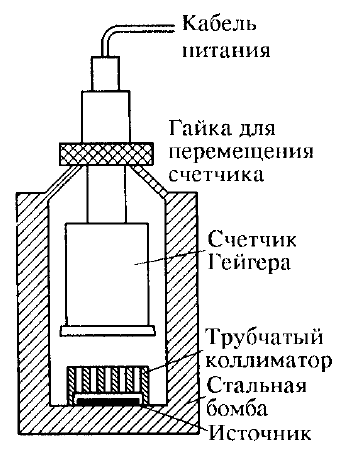
\includegraphics[scale = 0.4]{Workplace1}
    \centering
    \caption{Установка для измерения пробега $\alpha$-частиц с помощью торцевого счётчика Гейгера}
    \label{img:work1}
\end{figure}

\begin{figure}[H]
    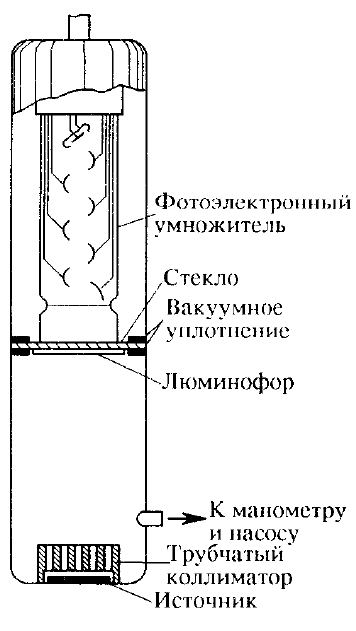
\includegraphics[scale = 0.4]{Workplace2}
    \centering
    \caption{Установка для измерения пробега $\alpha$-частиц с помощью сцинтилляционного счётчика}
    \label{img:work2}
\end{figure}

\begin{figure}[H]
    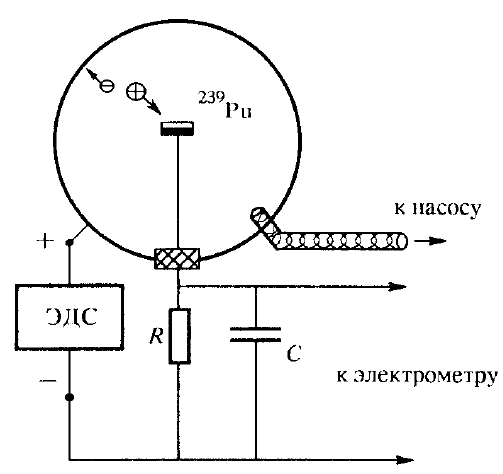
\includegraphics[scale = 0.4]{Workplace3}
    \centering
    \caption{Схема устройства ионизационной камеры}
    \label{img:work1}
\end{figure}

\parag {Ход работы} ~\\

\point Для начала воспользуемся счетчиком Гейгера. Снимем зависимость скорости счёта от расстояния $x$ от источника до приёмника. Результаты представлены в таблице \ref{tab:geig}.

\begin{table}[H]
    \centering
    \begin{tabular}{|c|c|c|c|c|c|c|c|c|}
        \hline
        $t$, с & 70.218 & 40.162 & 40.212 & 44.857 & 76.341 & 125.074 & 120.178 & 40.209 \\ \hline
        $N$ & 907 & 657 & 603 & 612 & 506 & 42 & 26 & 581 \\ \hline
        $x$, мм & 10.0 & 12.0 & 14.0 & 16.0 & 18.0 & 20.0 & 25.0 & 15.0 \\ \hline
    \end{tabular}
    \\~\\
    \begin{tabular}{|c|c|c|c|c|c|c|c|c|}
        \hline
        $t$, с & 40.206 & 40.206 & 40.584 & 51.685 & 119.884 & 119.975 & 120.123 \\ \hline
        $N$ & 568 & 544 & 505 & 502 & 339 & 108 & 47 \\ \hline
        $x$, мм & 15.5 & 16.5 & 17.0 & 17.5 & 18.5 & 19.0 & 19.5 \\ \hline
    \end{tabular}
    \caption {Измерения на счётчике Гейгера}
    \label{tab:geig}
\end{table}

\point Построим график $\dfrac{N}{t} (x)$ и $\dfrac{d (N/t)}{dx} (x)$ (см. рис. \ref{img:geig}). Определим по нем средний и экстраполированный пробег $\alpha$-частиц.

Получаем: 

\begin{align*}
    R_{ср} &\approx 18 ~ мм \\
    R_э &= 19.2 \pm 1.2 ~ мм
\end{align*}

Т.~к. $p_{атм} = 100$ кПа, т.~е. плотность воздуха $\rho \approx 1.184 \cdot 10^{-3}~\dfrac{г}{см^3}$, то можно перевести величины в $\dfrac{г}{см^2}$:

\begin{align*}
    R_{ср} &\approx 2.1 \cdot 10^{-3} & \dfrac{г}{см^2} \\
    R_э &= (2.27 \pm 0.14) ~ \cdot 10^{-3} & \dfrac{г}{см^2}
\end{align*}

\begin{figure}[H]
    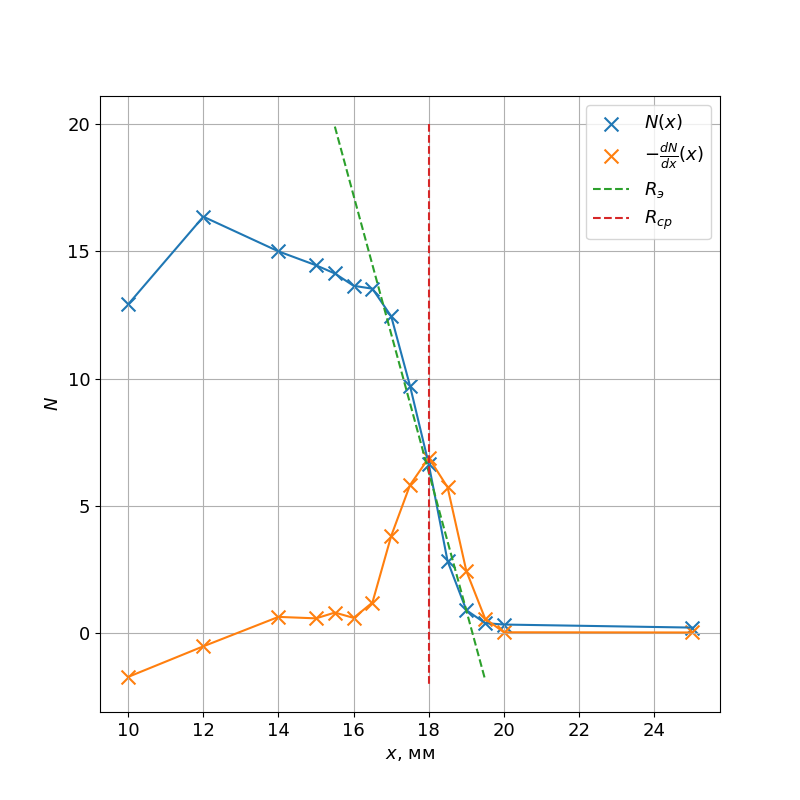
\includegraphics[scale = 0.6]{geiger.png}
    \centering
    \caption{График $N(x)$}
    \label{img:geig}
\end{figure}

\point Теперь снимем данные с помощью сцинтилляционного счётчика. Снимем зависимость $N(p)$, результат занесем в таблицу \ref{tab:sc}.

\begin{table}[!h]
    \centering
    \begin{tabular}{|c|c|c|c|c|c|c|c|c|c|c|c|c|}
        \hline
        $\Delta p$, мм.~рт.~ст. & 10 & 20 & 30 & 40 & 50 & 75 & 100 & 125 & 150 & 175 & 200 & 225\\ \hline
        $N$ & 3601 & 3455 & 3344 & 3314 & 2975 & 2714 & 2233 & 1774 & 1242 & 717 & 409 & 180\\ \hline
        $t$, с & 10 & 10 & 10 & 10 & 10 & 10 & 10 & 10 & 10 & 10 & 10 & 10\\ \hline
    \end{tabular}
    \\~\\
    \begin{tabular}{|c|c|c|c|c|c|c|c|c|c|c|c|}
        \hline
        $\Delta p$, мм.~рт.~ст. & 250 & 275 & 300 & 325 & 190 & 210 & 240 & 260 & 290 & 310 & 340\\ \hline
        $N$ & 93 & 64 & 16 & 3 & 680 & 294 & 119 & 87 & 59 & 7 & 5\\ \hline
        $t$, с & 10 & 10 & 10 & 10 & 10 & 10 & 10 & 10 & 10 & 10 & 10\\ \hline
    \end{tabular}
    \caption {Измерения на сцинтилляционном счётчике}
    \label{tab:sc}
\end{table}

\point Построим график $N (p)$, где $p = p_{атм} - \Delta p$, $p_{атм} = 750$~мм.~рт.~ст. Найдём, аналогично предыдущему пункту, $p_{ср}$ и $p_э$. Получаем:

\begin{align*}
    p_{ср} &\approx 147 ~ мм.~рт.~ст.  \\
    p_э &= (228 \pm 41) ~ мм.~рт.~ст.
\end{align*}

\begin{figure}[!h]
    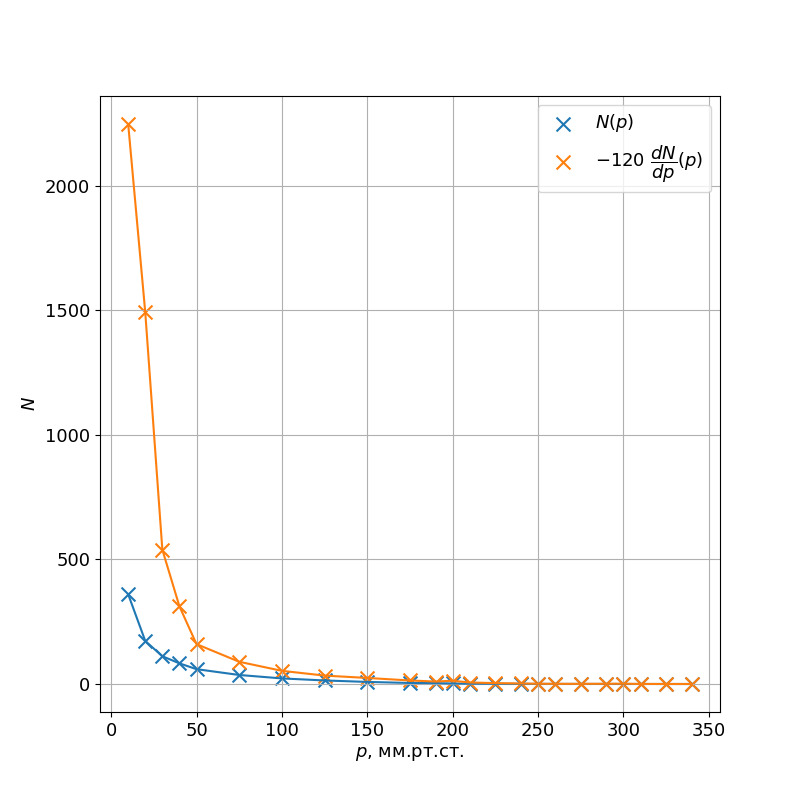
\includegraphics[scale = 0.6]{sc.png}
    \centering
    \caption{График $N(p)$}
    \label{img:sc}
\end{figure}

\point Пересчитаем пробег к $R$ при $p = 760$~мм.~рт.~ст. и $T = 288$ К. Учтём, что общая длина установки $9$ см.

% Коммент Андрея Вязовцева, студента ФРТК, автора оригинальной работы, с которой был подчистую скатан первый пункт этой лабы:
%"""
% Ну и дерьмо редкостое получилось. И да, продублирую: 
% Интересно, для кого я пишу это в шесть часов ночи? Напиши, если реально читаешь это.
%"""
%
% P.S про дерьмо поддерживаю. Лаба -- редкостная херня

\begin{align*}
    R_{ср} &\approx 17 ~ мм = 2 \cdot 10^{-3} ~ \dfrac{г}{см^2} \\
    R_э &= (27 \pm 6) ~ мм = (3.2 \pm 0.7) \cdot 10^{-3} ~ \dfrac{г}{см^2}
\end{align*}

\point Отсюда найдём толщину слюды:

\[
    l = 1.2 \cdot (R_{II} - R_{I}) = (10 \pm 7) \cdot 10^{-3} ~ \dfrac{г}{см^2}
\]

\point Вычислим по формуле \eqref{eq:sc} энегрию $\alpha$-частиц:

\[
    E = (4 \pm 1) ~МэВ
\]

Табличное значени -- $E = 5.15$ МэВ. Таким образом, полученные данные совпадают с табличными в рамках погрешности.

\point Приступим к измерениям с помощью ионизационной камеры. Исследуем зависимость $I(p)$. Результаты представлены в таблице \ref{tab:ion}.

\begin{table}[!h]
    \centering
    \begin{tabular}{|c|c|c|c|c|c|c|c|c|c|c|}
        \hline
        $\Delta p$, ~мм.~рт.~ст. & 30 & 50 & 75 & 100 & 125 & 150 & 178 & 200 & 225 & 250\\ \hline
        $I$, пА & 25 & 55 & 92 & 125 & 166 & 203 & 242 & 274 & 322 & 362\\ \hline
    \end{tabular}
    \\~\\
    \begin{tabular}{|c|c|c|c|c|c|c|c|c|c|}
        \hline
        $\Delta p$, ~мм.~рт.~ст. & 275 & 300 & 325 & 350 & 375 & 400 & 425 & 450 & 475\\ \hline
        $I$, пА & 408 & 450 & 492 & 538 & 585 & 630 & 685 & 725 & 778\\ \hline
    \end{tabular}
    \\~\\
    \begin{tabular}{|c|c|c|c|c|c|c|c|c|c|c|c|}
        \hline
        $\Delta p$, ~мм.~рт.~ст. & 500 & 530 & 550 & 575 & 600 & 625 & 650 & 675 & 700 & 725 & 750\\ \hline
        $I$, пА & 826 & 875 & 900 & 914 & 916 & 915 & 908 & 906 & 897 & 891 & 890\\ \hline
    \end{tabular}
    \caption {Метод ионизационной камеры}
    \label{tab:ion}
\end{table}

\point Изобразим зависимость на графике (рис. \ref{img:ion}). 

\begin{figure}[h]
    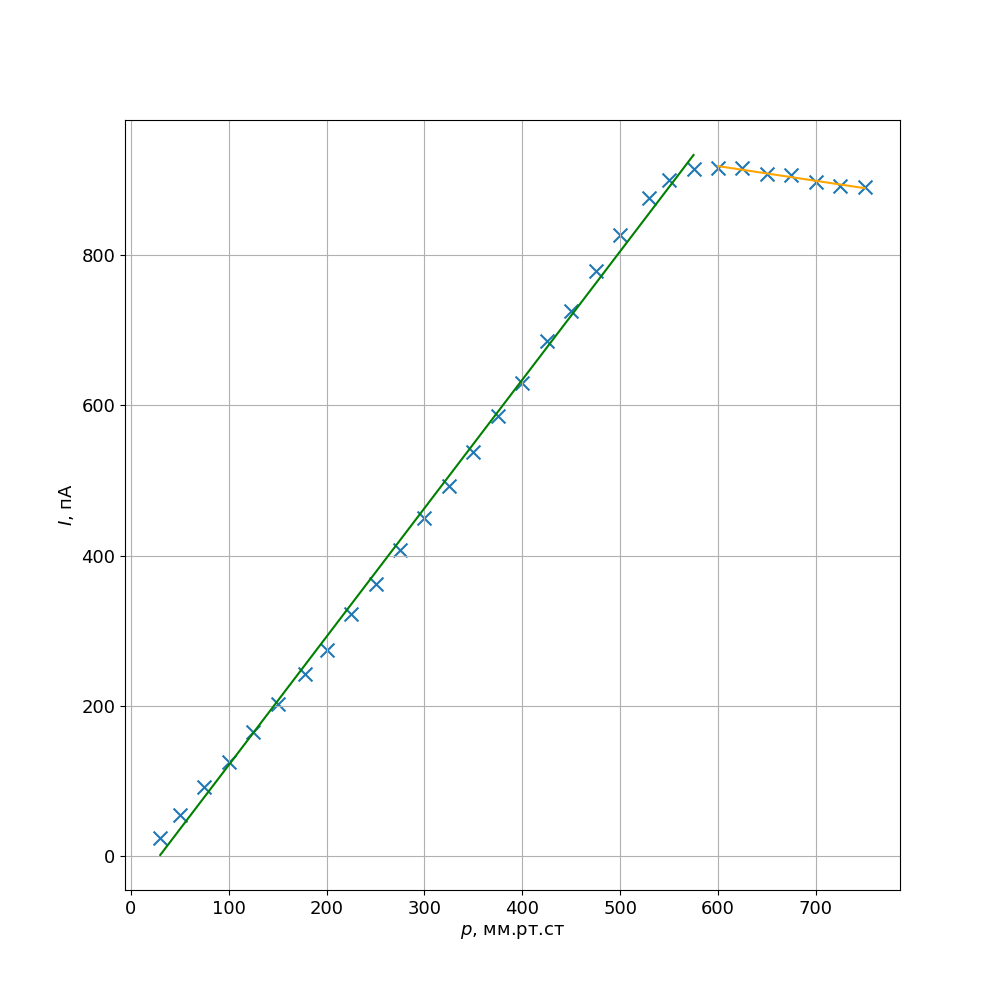
\includegraphics[scale = 0.6]{ion.png}
    \centering
    \caption{Зависимость $I(p)$}
    \label{img:ion}
\end{figure}

\point Из графика находим, что:

\[
    p_э = (569 \pm 10) ~мм.~рт.~ст.
\]

\point Далее найдём величины из предыдущих пунктов. Учтём, что $0.5$ см и $10$ см --- диаметры первого и второго электродов. 

\begin{align*}
    R_э &= (3.40 \pm 0.07) \cdot 10^{-3} ~ \dfrac{г}{см^2} \\
    E & = (4.8 \pm 0.1) ~МэВ
\end{align*}

\parag {Заключение} ~\\
В ходе лабораторной работы был измерен пробег $\alpha$-частиц в воздухе двумя способами и определена энергию частиц. Данные совпали с табличными по порядку величины.

\end{document}
